\documentclass[8pt,aspectratio=169]{beamer}
\usetheme{Madrid}
\usecolortheme{seahorse}
\setbeamertemplate{navigation symbols}{}

% Packages
\usepackage{graphicx}
\usepackage{amsmath}
\usepackage{amssymb}
\usepackage{tcolorbox}
\usepackage{tikz}
\usetikzlibrary{positioning,arrows.meta}

% Custom colors matching our Python visualizations
\definecolor{mlblue}{RGB}{68,114,196}
\definecolor{mlgreen}{RGB}{68,160,68}
\definecolor{mlorange}{RGB}{255,127,14}
\definecolor{mlred}{RGB}{214,39,40}
\definecolor{mlpurple}{RGB}{139,90,155}

% Title
\title{Transformers: Understanding Parallel Intelligence}
\subtitle{From Zero to ChatGPT - A BSc Journey}
\author{Week 5: Transformers}
\date{}

\begin{document}

% Slide 1: Title
\begin{frame}
\titlepage
\end{frame}

% Slide 2: Learning Objectives
\begin{frame}{What You'll Learn Today}
\begin{columns}[T]
\column{0.48\textwidth}
\textbf{By the end of this lecture, you will:}
\begin{enumerate}
\item \textbf{Understand} how words become numbers (embeddings)
\item \textbf{Explain} why parallel beats sequential processing
\item \textbf{Calculate} attention scores between words
\item \textbf{Draw} the transformer architecture
\item \textbf{Identify} transformers in daily applications
\end{enumerate}

\vspace{5mm}
\textbf{Prerequisites:}
\begin{itemize}
\item Basic vector operations (dot product)
\item Matrix multiplication concept
\item No deep learning needed!
\end{itemize}

\column{0.48\textwidth}
\textbf{Your Learning Journey:}

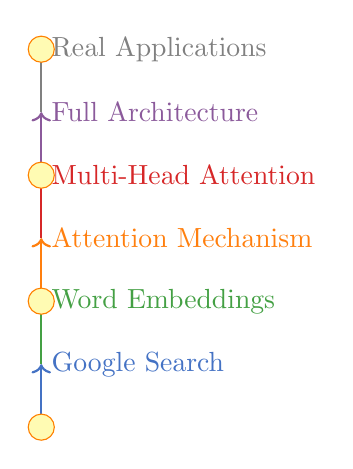
\begin{tikzpicture}[scale=0.8]
% Journey path
\draw[thick, ->, mlblue] (0,0) -- (0,1) node[right] {Google Search};
\draw[thick, ->, mlgreen] (0,1) -- (0,2) node[right] {Word Embeddings};
\draw[thick, ->, mlorange] (0,2) -- (0,3) node[right] {Attention Mechanism};
\draw[thick, ->, mlred] (0,3) -- (0,4) node[right] {Multi-Head Attention};
\draw[thick, ->, mlpurple] (0,4) -- (0,5) node[right] {Full Architecture};
\draw[thick, ->, gray] (0,5) -- (0,6) node[right] {Real Applications};

% Checkpoints
\foreach \y in {0,2,4,6} {
    \node[circle, fill=yellow!30, draw=orange] at (0,\y) {};
}
\end{tikzpicture}

\vspace{3mm}
\colorbox{yellow!20}{\parbox{0.9\columnwidth}{
\centering
\textbf{Interactive Elements:}\\
3 Checkpoints | 5 Exercises | 10 Visuals
}}
\end{columns}
\end{frame}

% ===========================================
% PART 1: THE CHALLENGE (5 slides)
% ===========================================

% Slide 3: The Google Search Experience
\begin{frame}{How Google Reads Your Mind}
\begin{columns}[T]
\column{0.48\textwidth}
\textbf{Try this:} Type in Google: ``How do transformers...''

\vspace{3mm}
\textbf{Google instantly suggests:}
\begin{itemize}
\item ``...work in machine learning''
\item ``...process language''
\item ``...learn from data''
\end{itemize}

\vspace{3mm}
\textbf{The Mystery:}
\begin{itemize}
\item Google reads ALL your words at once
\item Not word-by-word like old systems
\item Understands context instantly
\end{itemize}

\column{0.48\textwidth}
\begin{center}
\begin{tcolorbox}[colback=white,colframe=gray!75!black,width=0.9\columnwidth]
\texttt{How do transformers}\\[2mm]
\hrule\vspace{2mm}
{\small\color{gray}
\texttt{...work in machine learning}\\
\texttt{...process language}\\
\texttt{...learn from data}\\
\texttt{...handle attention}\\
}
\end{tcolorbox}
\end{center}

\vspace{3mm}
\begin{tcolorbox}[colback=yellow!10!white,colframe=orange!75!black]
\textbf{Question:} How does it understand whole sentences simultaneously?
\end{tcolorbox}
\end{columns}
\end{frame}

% Slide 4: Words as Coordinates in Space
\begin{frame}{Discovery 1: Words Live in Space}
\begin{columns}[T]
\column{0.48\textwidth}
\textbf{Think about GPS coordinates:}
\begin{itemize}
\item Paris: (48.8N, 2.3E, 35m altitude)
\item London: (51.5N, 0.1W, 11m altitude)
\item Similar cities are nearby in space
\end{itemize}

\vspace{3mm}
\textbf{Words work the same way!}
\begin{itemize}
\item ``cat'': [0.7, 0.2, 0.5] in meaning space
\item ``dog'': [0.8, 0.3, 0.4] (nearby - similar!)
\item ``car'': [0.1, 0.9, 0.2] (far - different!)
\end{itemize}

\vspace{3mm}
\textbf{This is called:} \colorbox{mlblue!20}{Word Embeddings}

\column{0.48\textwidth}
\begin{center}
\includegraphics[width=0.95\columnwidth]{../figures/word_embeddings_3d.pdf}
\end{center}
\end{columns}
\end{frame}

% Slide 5: Every Word Connects to Every Other
\begin{frame}{Discovery 2: Every Word Connects to Every Other}
\begin{columns}[T]
\column{0.48\textwidth}
\textbf{In a sentence, every word ``talks'' to every other:}

\vspace{3mm}
\textbf{Example:} ``The cat sat on mat''
\begin{itemize}
\item ``cat'' checks all other words
\item ``sat'' looks at subject and location
\item ``mat'' knows what's on it
\end{itemize}

\vspace{5mm}
\textbf{Total connections:} $n \times n$
\begin{itemize}
\item 5 words = 25 connections
\item 100 words = 10,000 connections!
\end{itemize}

\column{0.48\textwidth}
\begin{center}
\includegraphics[width=0.95\columnwidth]{../figures/parallel_connections_3d.pdf}
\end{center}

\vspace{3mm}
\colorbox{mlgreen!20}{\parbox{0.9\columnwidth}{
\centering
\textbf{Key Insight:}\\
Transformers compute ALL connections\\
SIMULTANEOUSLY!
}}
\end{columns}
\end{frame}

% Slide 6: The Problem - Information Overload
\begin{frame}{The Problem: Information Overload}
\begin{columns}[T]
\column{0.48\textwidth}
\textbf{Challenge:} Too much information!

\vspace{3mm}
\textbf{Sentence:} ``The bank by the river bank''
\begin{itemize}
\item First ``bank'' = financial institution
\item Second ``bank'' = river edge
\item How does the model know?
\end{itemize}

\vspace{5mm}
\textbf{Information explosion:}
\begin{itemize}
\item Every word sends signals to all others
\item Most connections are noise
\item Need to focus on what matters
\end{itemize}

\column{0.48\textwidth}
\begin{center}
\includegraphics[width=0.95\columnwidth]{../figures/information_overload_3d.pdf}
\end{center}

\vspace{3mm}
\colorbox{mlred!20}{\parbox{0.9\columnwidth}{
\centering
\textbf{Problem:} With 100 words,\\
99\% of connections are irrelevant!
}}
\end{columns}
\end{frame}

% ===========================================
% PART 2: THE INSIGHT (5 slides)
% ===========================================

% Slide 7: First Attempt
\begin{frame}{First Attempt: Connect Everything}
\textbf{Early 2010s approach: Just connect everything!}

\vspace{5mm}
\begin{center}
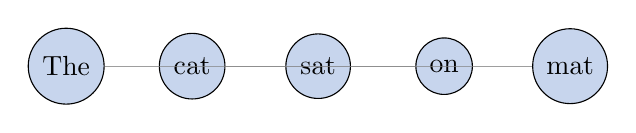
\begin{tikzpicture}[scale=0.8]
% Words
\node[circle,draw,fill=mlblue!30] (w1) at (0,0) {The};
\node[circle,draw,fill=mlblue!30] (w2) at (2,0) {cat};
\node[circle,draw,fill=mlblue!30] (w3) at (4,0) {sat};
\node[circle,draw,fill=mlblue!30] (w4) at (6,0) {on};
\node[circle,draw,fill=mlblue!30] (w5) at (8,0) {mat};

% Draw all connections
\foreach \i in {1,2,3,4,5} {
    \foreach \j in {1,2,3,4,5} {
        \ifnum\i<\j
            \draw[gray,opacity=0.3] (w\i) -- (w\j);
        \fi
    }
}
\end{tikzpicture}
\end{center}

\vspace{5mm}
\textbf{Results:}
\begin{itemize}
\item \checkmark Works for short sentences
\item $\times$ Fails on long text
\item $\times$ Can't distinguish important from noise
\end{itemize}
\end{frame}

% Slide 8: Computing All Relationships
\begin{frame}{Computing All Relationships}
\begin{columns}[T]
\column{0.48\textwidth}
\textbf{What happens with full connections:}

\vspace{3mm}
\textbf{Step 1:} Every word becomes a vector
\begin{itemize}
\item ``cat'' → [0.7, 0.2, 0.5]
\item ``sat'' → [0.3, 0.8, 0.4]
\item ``mat'' → [0.6, 0.1, 0.7]
\end{itemize}

\vspace{3mm}
\textbf{Step 2:} Compute all dot products
\begin{itemize}
\item cat · sat = 0.59
\item cat · mat = 0.87
\item sat · mat = 0.52
\end{itemize}

\vspace{3mm}
\textbf{Step 3:} Average everything
Result: Information soup!

\column{0.48\textwidth}
\begin{center}
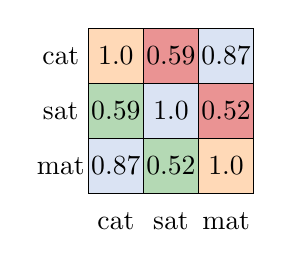
\begin{tikzpicture}[scale=0.7]
% Matrix visualization
\draw[fill=mlblue!20] (0,0) rectangle (1,1);
\draw[fill=mlgreen!40] (1,0) rectangle (2,1);
\draw[fill=mlorange!30] (2,0) rectangle (3,1);
\draw[fill=mlgreen!40] (0,1) rectangle (1,2);
\draw[fill=mlblue!20] (1,1) rectangle (2,2);
\draw[fill=mlred!50] (2,1) rectangle (3,2);
\draw[fill=mlorange!30] (0,2) rectangle (1,3);
\draw[fill=mlred!50] (1,2) rectangle (2,3);
\draw[fill=mlblue!20] (2,2) rectangle (3,3);

% Labels
\node at (-0.5,0.5) {mat};
\node at (-0.5,1.5) {sat};
\node at (-0.5,2.5) {cat};
\node at (0.5,-0.5) {cat};
\node at (1.5,-0.5) {sat};
\node at (2.5,-0.5) {mat};

% Values
\node at (0.5,2.5) {1.0};
\node at (1.5,2.5) {0.59};
\node at (2.5,2.5) {0.87};
\node at (0.5,1.5) {0.59};
\node at (1.5,1.5) {1.0};
\node at (2.5,1.5) {0.52};
\node at (0.5,0.5) {0.87};
\node at (1.5,0.5) {0.52};
\node at (2.5,0.5) {1.0};
\end{tikzpicture}
\end{center}

\colorbox{yellow!20}{\parbox{0.9\columnwidth}{
All relationships computed but no focus!
}}
\end{columns}
\end{frame}

% Slide 9: SUCCESS on Simple Cases
\begin{frame}{SUCCESS! (On Simple Cases)}
\begin{columns}[T]
\column{0.48\textwidth}
\textbf{When it works:}

\vspace{3mm}
\textbf{Short, clear sentences:}
\begin{itemize}
\item ``Dogs love bones'' \checkmark
\item ``Paris is beautiful'' \checkmark
\item ``Water is wet'' \checkmark
\end{itemize}

\vspace{5mm}
\textbf{Why it works here:}
\begin{itemize}
\item Few connections (9 total for 3 words)
\item All connections matter
\item No ambiguity
\end{itemize}

\column{0.48\textwidth}
\begin{center}
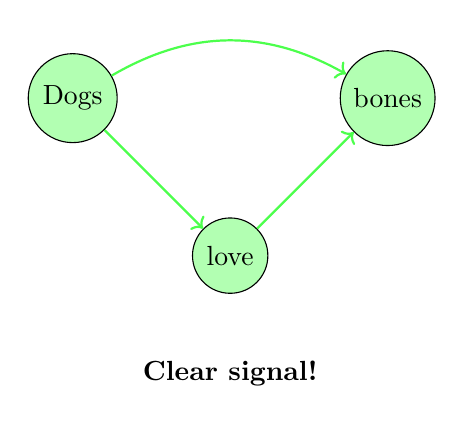
\begin{tikzpicture}[scale=1]
% Success visualization
\node[circle,draw,fill=green!30] (s1) at (0,2) {Dogs};
\node[circle,draw,fill=green!30] (s2) at (2,0) {love};
\node[circle,draw,fill=green!30] (s3) at (4,2) {bones};

\draw[thick,green!70,->] (s1) -- (s2);
\draw[thick,green!70,->] (s2) -- (s3);
\draw[thick,green!70,->] (s1) to[bend left] (s3);

\node at (2,-1.5) {\textbf{Clear signal!}};
\end{tikzpicture}
\end{center}

\vspace{5mm}
\colorbox{green!20}{\parbox{0.9\columnwidth}{
\centering
\textbf{Success Rate:} 95\% on 3-5 word sentences
}}
\end{columns}
\end{frame}

% Slide 10: FAILURE - Signal Lost in Noise
\begin{frame}{FAILURE: Signal Lost in Noise}
\begin{columns}[T]
\column{0.48\textwidth}
\textbf{When it fails:}

\vspace{3mm}
\textbf{Real-world sentence:}
``The \textcolor{red}{bank} agreed to provide a loan for the house by the river \textcolor{red}{bank} after reviewing the application that the customer submitted last Tuesday.''

\vspace{3mm}
\textbf{Problems:}
\begin{itemize}
\item 20 words = 400 connections!
\item ``bank'' (financial) vs ``bank'' (river)
\item Long-distance dependencies
\item Most connections are noise
\end{itemize}

\column{0.48\textwidth}
\begin{center}
\includegraphics[width=0.95\columnwidth]{../figures/noise_visualization.pdf}
\end{center}

\vspace{3mm}
\colorbox{red!20}{\parbox{0.9\columnwidth}{
\centering
\textbf{Failure Rate:} 60\% on 15+ word sentences\\
Signal drowned in noise!
}}
\end{columns}
\end{frame}

% Slide 11: How Do Humans Actually Read?
\begin{frame}{How Do Humans Actually Read?}
\begin{columns}[T]
\column{0.48\textwidth}
\textbf{Eye-tracking studies reveal:}

\vspace{3mm}
\textbf{Humans DON'T read every word equally!}

\vspace{3mm}
Reading: ``The quick brown fox jumps''
\begin{itemize}
\item Focus on ``fox'' and ``jumps''
\item Skim ``the'' and ``brown''
\item Context determines focus
\end{itemize}

\vspace{5mm}
\textbf{Human attention is:}
\begin{itemize}
\item Selective (ignore irrelevant)
\item Contextual (meaning-based)
\item Efficient (focus on key parts)
\end{itemize}

\column{0.48\textwidth}
\begin{center}
\includegraphics[width=0.95\columnwidth]{../figures/attention_heatmap.pdf}
\end{center}

\vspace{3mm}
\colorbox{mlpurple!20}{\parbox{0.9\columnwidth}{
\centering
\textbf{Key Insight:}\\
We need SELECTIVE attention,\\
not full connections!
}}
\end{columns}
\end{frame}

% ===========================================
% PART 3: THE SOLUTION (8 slides)
% ===========================================

% Slide 12: The Hypothesis - Selective Attention
\begin{frame}{The Hypothesis: Selective Attention}
\begin{columns}[T]
\column{0.48\textwidth}
\textbf{The Breakthrough (2017):}

\vspace{3mm}
Instead of connecting everything equally,\\
\textbf{learn WHICH connections matter!}

\vspace{5mm}
\textbf{Attention Mechanism:}
\begin{enumerate}
\item Compute importance scores
\item Focus on high scores
\item Ignore low scores
\end{enumerate}

\vspace{5mm}
\textbf{Like a spotlight:}
\begin{itemize}
\item Bright on important words
\item Dim on filler words
\item Adjustable based on context
\end{itemize}

\column{0.48\textwidth}
\begin{center}
\includegraphics[width=0.95\columnwidth]{../figures/attention_spotlight_3d.pdf}
\end{center}

\vspace{3mm}
\colorbox{mlorange!20}{\parbox{0.9\columnwidth}{
\centering
\textbf{Attention} = Learning what to focus on
}}
\end{columns}
\end{frame}

% Slide 13: Attention as Percentages
\begin{frame}{Breaking It Down: Attention as Percentages}
\begin{columns}[T]
\column{0.48\textwidth}
\textbf{Example:} ``The cat sat on mat''

\vspace{3mm}
\textbf{When processing ``sat'':}
\begin{itemize}
\item 40\% attention to ``cat'' (who sat?)
\item 30\% attention to ``mat'' (where?)
\item 20\% attention to ``on'' (relation)
\item 5\% to ``The'' (not important)
\item 5\% to itself
\end{itemize}

\vspace{5mm}
\textbf{These percentages:}
\begin{itemize}
\item Always sum to 100\%
\item Change for each word
\item Learned from data
\end{itemize}

\column{0.48\textwidth}
\begin{center}
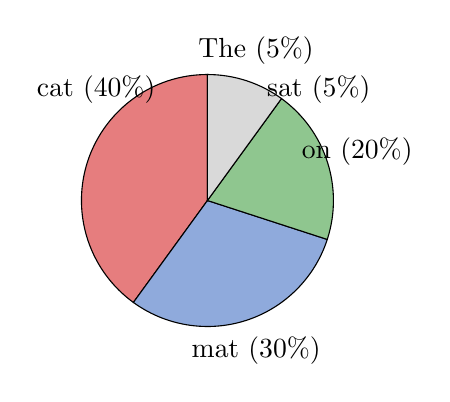
\begin{tikzpicture}[scale=0.8]
% Pie chart for attention
\draw[fill=mlred!60] (0,0) -- (0,2) arc (90:234:2) -- cycle;
\draw[fill=mlblue!60] (0,0) -- (234:2) arc (234:342:2) -- cycle;
\draw[fill=mlgreen!60] (0,0) -- (342:2) arc (342:414:2) -- cycle;
\draw[fill=gray!30] (0,0) -- (414:2) arc (414:450:2) -- cycle;
\draw[fill=gray!20] (0,0) -- (450:2) arc (450:450:2) -- cycle;

% Labels
\node at (135:2.5) {cat (40\%)};
\node at (288:2.5) {mat (30\%)};
\node at (378:2.5) {on (20\%)};
\node at (432:2.5) {The (5\%)};
\node at (45:2.5) {sat (5\%)};
\end{tikzpicture}
\end{center}

\vspace{3mm}
\colorbox{yellow!20}{\parbox{0.9\columnwidth}{
\centering
\textbf{Softmax} ensures percentages\\
always total 100\%
}}
\end{columns}
\end{frame}

% Slide 14: The Math - How Similar Are Two Words?
\begin{frame}{The Math: How Similar Are Two Words?}
\begin{columns}[T]
\column{0.48\textwidth}
\textbf{Measuring similarity with angles:}

\vspace{3mm}
\textbf{Dot Product Formula:}
$$\text{similarity} = \vec{A} \cdot \vec{B} = |\vec{A}| \times |\vec{B}| \times \cos(\theta)$$

\vspace{3mm}
\textbf{What this means:}
\begin{itemize}
\item Same direction: $\cos(0^\circ) = 1$ (max similar)
\item Perpendicular: $\cos(90^\circ) = 0$ (unrelated)
\item Opposite: $\cos(180^\circ) = -1$ (opposite)
\end{itemize}

\vspace{3mm}
\textbf{Example:}
\begin{itemize}
\item cat · dog = 0.8 (similar animals)
\item cat · car = 0.1 (very different)
\end{itemize}

\column{0.48\textwidth}
\begin{center}
\includegraphics[width=0.95\columnwidth]{../figures/dot_product_visualization.pdf}
\end{center}

\colorbox{mlblue!20}{\parbox{0.9\columnwidth}{
\centering
Dot product = Semantic similarity
}}
\end{columns}
\end{frame}

% Slide 15: Query, Key, Value
\begin{frame}{The Three Questions: Query, Key, Value}
\begin{columns}[T]
\column{0.48\textwidth}
\textbf{For each word, we ask 3 questions:}

\vspace{3mm}
\textbf{1. Query (Q):} ``What am I looking for?''
\begin{itemize}
\item Cat's query: ``Who performed action on me?''
\end{itemize}

\vspace{3mm}
\textbf{2. Key (K):} ``What do I offer?''
\begin{itemize}
\item Sat's key: ``I am an action verb''
\end{itemize}

\vspace{3mm}
\textbf{3. Value (V):} ``What information do I provide?''
\begin{itemize}
\item Sat's value: ``Past tense sitting action''
\end{itemize}

\vspace{3mm}
\textbf{Matching:} Q·K determines attention weight

\column{0.48\textwidth}
\begin{center}
\includegraphics[width=0.95\columnwidth]{../figures/qkv_transformation_3d.pdf}
\end{center}

\colorbox{mlorange!20}{\parbox{0.9\columnwidth}{
\centering
\textbf{QKV} transforms each word\\
into searcher, identifier, and content
}}
\end{columns}
\end{frame}

% Slide 15b: QKV Visualization (Larger)
\begin{frame}{Query, Key, Value Transformation}
\begin{center}
\includegraphics[width=0.55\textwidth]{../figures/qkv_transformation_3d.pdf}
\end{center}
\colorbox{mlorange!20}{\parbox{0.45\textwidth}{
\centering\small
\textbf{Three roles:} Q=Query, K=Key, V=Value
}}
\end{frame}

% Slide 15c: QKV Visualization (Graphviz)
\begin{frame}{Query, Key, Value Transformation (Flow Diagram)}
\begin{center}
\includegraphics[width=0.85\textwidth]{../figures/qkv_transformation_graphviz.pdf}
\end{center}
\end{frame}

% Slide 16: Step-by-Step Attention
\begin{frame}{Step-by-Step: Computing Attention}
\begin{center}
\includegraphics[width=0.6\textwidth]{../figures/attention_flow_diagram.pdf}
\end{center}
\colorbox{mlgreen!20}{\parbox{0.7\textwidth}{
\centering\small
\textbf{1.} Q·K \textbf{2.} Softmax \textbf{3.} Weight V \textbf{4.} Sum
}}
\end{frame}

% Slide 16b: Attention Steps (Graphviz)
\begin{frame}{Computing Attention: Detailed Flow}
\begin{center}
\includegraphics[width=0.95\textwidth]{../figures/attention_steps_graphviz.pdf}
\end{center}
\end{frame}

% Slide 16c: Attention Example (Graphviz)
\begin{frame}{Computing Attention: Concrete Example}
\vspace{-5mm}
\begin{center}
\includegraphics[width=0.38\textwidth]{../figures/attention_example_graphviz.pdf}
\end{center}
\end{frame}

% Slide 17: Multiple Perspectives
\begin{frame}{Multiple Perspectives: 4 Different Experts}
\begin{columns}[T]
\column{0.48\textwidth}
\textbf{Multi-Head Attention:}

\vspace{3mm}
Like having 4 specialist readers:

\vspace{3mm}
\textbf{Head 1:} Grammar Expert
\begin{itemize}
\item Subject-verb agreement
\item Sentence structure
\end{itemize}

\textbf{Head 2:} Meaning Expert
\begin{itemize}
\item Semantic relationships
\item Word meanings
\end{itemize}

\textbf{Head 3:} Position Expert
\begin{itemize}
\item Word order
\item Distance relationships
\end{itemize}

\textbf{Head 4:} Context Expert
\begin{itemize}
\item Broader context
\item Document theme
\end{itemize}

\column{0.48\textwidth}
\begin{center}
\includegraphics[width=0.95\columnwidth]{../figures/multi_head_3d.pdf}
\end{center}

\vspace{3mm}
\colorbox{mlpurple!20}{\parbox{0.9\columnwidth}{
\centering
\textbf{4 heads} = 4 different viewpoints\\
Combined for complete understanding
}}
\end{columns}
\end{frame}

% ===========================================
% PART 4: THE ARCHITECTURE (5 slides)
% ===========================================

% Slide 18: The Speed Revolution
\begin{frame}{The Speed Revolution: Everything at Once}
\begin{columns}[T]
\column{0.48\textwidth}
\textbf{Old way (RNN):} Sequential
\begin{itemize}
\item Process word 1, then 2, then 3...
\item 100 words = 100 time steps
\item Like reading one letter at a time
\end{itemize}

\vspace{5mm}
\textbf{New way (Transformer):} Parallel
\begin{itemize}
\item Process ALL words simultaneously
\item 100 words = 1 time step!
\item Like seeing whole page instantly
\end{itemize}

\vspace{5mm}
\textbf{Speed improvement:}
\begin{itemize}
\item Training: 90 days → 1 day
\item Inference: 10 seconds → 0.1 seconds
\end{itemize}

\column{0.48\textwidth}
\begin{center}
\includegraphics[width=0.95\columnwidth]{../figures/parallel_vs_sequential.pdf}
\end{center}
\end{columns}
\end{frame}

% Slide 19: Positional Encoding
\begin{frame}{Preserving Order: Where Words Live}
\begin{columns}[T]
\column{0.48\textwidth}
\textbf{Problem:} Parallel loses word order!

\vspace{3mm}
``Dog bites man'' vs ``Man bites dog''
\begin{itemize}
\item Same words, different meaning
\item Position matters!
\end{itemize}

\vspace{5mm}
\textbf{Solution: Positional Encoding}
\begin{itemize}
\item Add position information
\item Use sine/cosine waves
\item Different frequency for each dimension
\end{itemize}

\vspace{3mm}
\textbf{Like GPS for words:}
\begin{itemize}
\item Word + Position = Unique identity
\item Model knows where each word is
\end{itemize}

\vspace{3mm}
\colorbox{mlblue!20}{\parbox{0.8\columnwidth}{
\centering
Position encoding =\\Word's address
}}

\column{0.48\textwidth}
\begin{center}
\includegraphics[width=0.75\columnwidth]{../figures/positional_encoding_3d.pdf}
\end{center}
\end{columns}
\end{frame}

% Slide 20: Residual Connections
\begin{frame}{The Highway: Residual Connections}
\begin{columns}[T]
\column{0.48\textwidth}
\textbf{Problem with deep networks:}
\begin{itemize}
\item Information gets lost/distorted
\item Like telephone game
\item Each layer adds noise
\end{itemize}

\vspace{5mm}
\textbf{Solution: Skip Connections}
\begin{itemize}
\item Create ``highways'' for information
\item Original signal preserved
\item Add refinements, don't replace
\end{itemize}

\vspace{5mm}
\textbf{Formula:}
$$\text{Output} = \text{Layer}(x) + x$$
Always keep original, add improvements

\column{0.48\textwidth}
\begin{center}
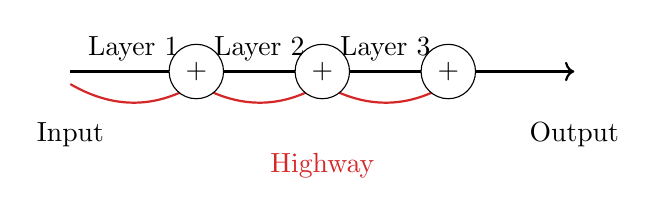
\begin{tikzpicture}[scale=0.8]
% Main path
\draw[thick,->] (0,0) -- (2,0) node[midway,above] {Layer 1};
\draw[thick,->] (2,0) -- (4,0) node[midway,above] {Layer 2};
\draw[thick,->] (4,0) -- (6,0) node[midway,above] {Layer 3};
\draw[thick,->] (6,0) -- (8,0);

% Skip connections (highways)
\draw[thick,mlred,->] (0,-0.2) to[bend right=30] (2,-0.2);
\draw[thick,mlred,->] (2,-0.2) to[bend right=30] (4,-0.2);
\draw[thick,mlred,->] (4,-0.2) to[bend right=30] (6,-0.2);

% Labels
\node at (0,-1) {Input};
\node at (8,-1) {Output};
\node[mlred] at (4,-1.5) {Highway};

% Addition points
\node[circle,draw,fill=white] at (2,0) {+};
\node[circle,draw,fill=white] at (4,0) {+};
\node[circle,draw,fill=white] at (6,0) {+};
\end{tikzpicture}
\end{center}

\vspace{5mm}
\colorbox{mlred!20}{\parbox{0.9\columnwidth}{
\centering
Residual = Original + Refinement\\
Never lose information!
}}
\end{columns}
\end{frame}

% Slide 21: Everything Together
\begin{frame}{Everything Together: The Transformer}
\begin{columns}[T]
\column{0.48\textwidth}
\textbf{The Complete Architecture:}

\vspace{3mm}
\textbf{1. Input:} Words → Embeddings + Position

\vspace{2mm}
\textbf{2. Attention Block:}
\begin{itemize}
\item Multi-head attention
\item Add \& normalize (residual)
\end{itemize}

\vspace{2mm}
\textbf{3. Feed-Forward Block:}
\begin{itemize}
\item Two linear layers
\item Add \& normalize (residual)
\end{itemize}

\vspace{2mm}
\textbf{4. Stack 12 times} (BERT) or 96 times (GPT-3)

\vspace{2mm}
\textbf{5. Output:} Next word prediction

\column{0.48\textwidth}
\begin{center}
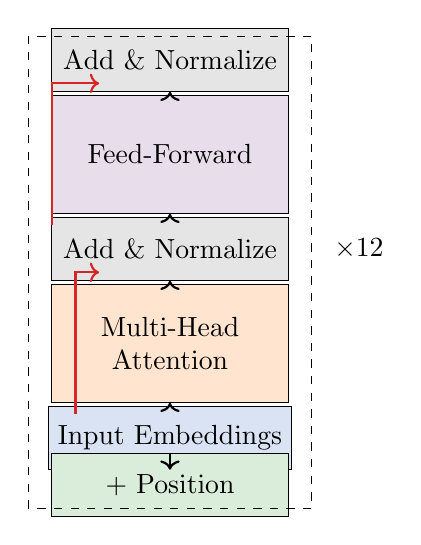
\begin{tikzpicture}[scale=0.6]
% Input
\node[draw,rectangle,fill=mlblue!20,minimum width=3cm,minimum height=0.8cm] (input) at (0,0) {Input Embeddings};

% Position
\node[draw,rectangle,fill=mlgreen!20,minimum width=3cm,minimum height=0.8cm] (pos) at (0,-1) {+ Position};

% Attention
\node[draw,rectangle,fill=mlorange!20,minimum width=3cm,minimum height=1.5cm,align=center] (attention) at (0,2) {Multi-Head\\Attention};

% Add & Norm
\node[draw,rectangle,fill=gray!20,minimum width=3cm,minimum height=0.8cm] (norm1) at (0,4) {Add \& Normalize};

% Feed-forward
\node[draw,rectangle,fill=mlpurple!20,minimum width=3cm,minimum height=1.5cm] (ff) at (0,6) {Feed-Forward};

% Add & Norm
\node[draw,rectangle,fill=gray!20,minimum width=3cm,minimum height=0.8cm] (norm2) at (0,8) {Add \& Normalize};

% Arrows
\draw[thick,->] (pos) -- (input);
\draw[thick,->] (input) -- (attention);
\draw[thick,->] (attention) -- (norm1);
\draw[thick,->] (norm1) -- (ff);
\draw[thick,->] (ff) -- (norm2);

% Residual connections
\draw[thick,mlred,->] (-2,0.5) -- (-2,3.5) -- (-1.5,3.5);
\draw[thick,mlred,->] (-2.5,4.5) -- (-2.5,7.5) -- (-1.5,7.5);

% Stack indicator
\draw[dashed] (-3,-1.5) rectangle (3,8.5);
\node at (4,4) {$\times 12$};
\end{tikzpicture}
\end{center}
\end{columns}
\end{frame}

% Slide 22: Proof It Works
\begin{frame}{Proof It Works: Real Results}
\begin{columns}[T]
\column{0.48\textwidth}
\textbf{Benchmark Results (2017-2024):}

\vspace{3mm}
\textbf{Translation (BLEU scores):}
\begin{itemize}
\item 2016 (RNN): 19.2
\item 2017 (Transformer): 28.4 \checkmark
\item 2024 (GPT-4): 35.1 \checkmark
\end{itemize}

\vspace{3mm}
\textbf{Question Answering:}
\begin{itemize}
\item Human performance: 89\%
\item BERT (2018): 93\% \checkmark
\item GPT-4 (2023): 96\% \checkmark
\end{itemize}

\vspace{3mm}
\textbf{Training Speed:}
\begin{itemize}
\item RNN: 3 months
\item Transformer: 1 day \checkmark
\end{itemize}

\column{0.48\textwidth}
\begin{center}
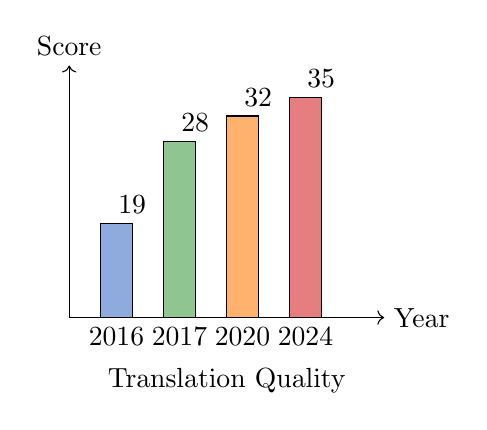
\begin{tikzpicture}[scale=0.8]
% Bar chart
\draw[->] (0,0) -- (5,0) node[right] {Year};
\draw[->] (0,0) -- (0,4) node[above] {Score};

% Bars
\draw[fill=mlblue!60] (0.5,0) rectangle (1,1.5) node[above] {19};
\draw[fill=mlgreen!60] (1.5,0) rectangle (2,2.8) node[above] {28};
\draw[fill=mlorange!60] (2.5,0) rectangle (3,3.2) node[above] {32};
\draw[fill=mlred!60] (3.5,0) rectangle (4,3.5) node[above] {35};

% Labels
\node at (0.75,-0.3) {2016};
\node at (1.75,-0.3) {2017};
\node at (2.75,-0.3) {2020};
\node at (3.75,-0.3) {2024};

\node at (2.5,-1) {Translation Quality};
\end{tikzpicture}
\end{center}

\vspace{3mm}
\colorbox{green!20}{\parbox{0.9\columnwidth}{
\centering
\textbf{Transformers:} State-of-the-art\\
on EVERY language task!
}}
\end{columns}
\end{frame}

% ===========================================
% PART 5: THE IMPACT (3 slides)
% ===========================================

% Slide 23: The Revolution
\begin{frame}{The Revolution: 2017-2024}
\begin{columns}[T]
\column{0.48\textwidth}
\textbf{Timeline of Breakthroughs:}

\vspace{3mm}
\textbf{2017:} Transformer paper
\begin{itemize}
\item ``Attention is All You Need''
\item 8 researchers at Google
\end{itemize}

\textbf{2018:} BERT
\begin{itemize}
\item Bidirectional understanding
\item Crushed 11 benchmarks
\end{itemize}

\textbf{2020:} GPT-3
\begin{itemize}
\item 175 billion parameters
\item Few-shot learning
\end{itemize}

\textbf{2023:} ChatGPT/GPT-4
\begin{itemize}
\item Conversation ability
\item 100M users in 2 months
\end{itemize}

\column{0.48\textwidth}
\begin{center}
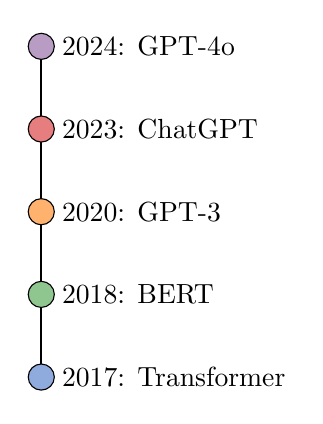
\begin{tikzpicture}[scale=0.7]
% Timeline
\draw[thick,->] (0,0) -- (0,6);

% Events
\node[circle,fill=mlblue!60,draw] at (0,0) {};
\node[right] at (0.2,0) {2017: Transformer};

\node[circle,fill=mlgreen!60,draw] at (0,1.5) {};
\node[right] at (0.2,1.5) {2018: BERT};

\node[circle,fill=mlorange!60,draw] at (0,3) {};
\node[right] at (0.2,3) {2020: GPT-3};

\node[circle,fill=mlred!60,draw] at (0,4.5) {};
\node[right] at (0.2,4.5) {2023: ChatGPT};

\node[circle,fill=mlpurple!60,draw] at (0,6) {};
\node[right] at (0.2,6) {2024: GPT-4o};
\end{tikzpicture}
\end{center}

\colorbox{mlpurple!20}{\parbox{0.9\columnwidth}{
\centering
7 years: From research paper\\
to 1 billion users!
}}
\end{columns}
\end{frame}

% Slide 24: Practice Problems
\begin{frame}{Practice Problems}
\begin{columns}[T]
\column{0.48\textwidth}
\textbf{Problem 1: Calculate Attention}

Given vectors:
\begin{itemize}
\item Query: [1, 0, 1]
\item Key1: [1, 1, 0]
\item Key2: [0, 1, 1]
\item Key3: [1, 0, 1]
\end{itemize}

Calculate:
\begin{enumerate}
\item Q · K for each key
\item Apply softmax
\item Which word gets most attention?
\end{enumerate}

\vspace{3mm}
\textbf{Problem 2: Multi-Head Design}

Design 3 attention heads for:
``The bank near the river bank''

What should each head focus on?

\column{0.48\textwidth}
\textbf{Problem 3: Architecture}

Draw transformer architecture for:
\begin{itemize}
\item 2-layer transformer
\item Show residual connections
\item Label each component
\end{itemize}

\vspace{5mm}
\textbf{Problem 4: Complexity}

For a 100-word sentence:
\begin{itemize}
\item How many attention scores?
\item Memory requirement?
\item Why is this $O(n^2)$?
\end{itemize}

\vspace{5mm}
\colorbox{yellow!20}{\parbox{0.9\columnwidth}{
\centering
\textbf{Solutions:} Available after lab session
}}
\end{columns}
\end{frame}

% Slide 25: Summary - The Three Core Principles
\begin{frame}{Summary: The Three Core Principles}
\begin{columns}[T]
\column{0.48\textwidth}
\textbf{1. Parallel Processing}
\begin{itemize}
\item All words processed simultaneously
\item 90x faster than sequential
\item Enables large-scale training
\end{itemize}

\vspace{3mm}
\textbf{2. Attention Mechanism}
\begin{itemize}
\item Focus on relevant connections
\item Learn what matters from data
\item Multiple perspectives (heads)
\end{itemize}

\vspace{3mm}
\textbf{3. Deep Architecture}
\begin{itemize}
\item Stack many layers (12-96)
\item Residual connections preserve info
\item Each layer refines understanding
\end{itemize}

\column{0.48\textwidth}
\begin{center}
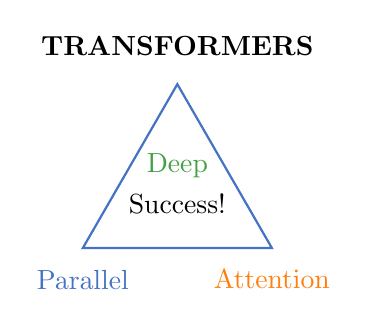
\begin{tikzpicture}[scale=0.8]
% Triangle of principles
\draw[thick,mlblue] (0,0) -- (3,0) -- (1.5,2.6) -- cycle;

% Labels
\node at (1.5,3.2) {\textbf{TRANSFORMERS}};
\node[mlblue] at (0,-0.5) {Parallel};
\node[mlorange] at (3,-0.5) {Attention};
\node[mlgreen] at (1.5,1.3) {Deep};

% Center
\node at (1.5,0.7) {Success!};
\end{tikzpicture}
\end{center}

\vspace{5mm}
\colorbox{mlgreen!20}{\parbox{0.9\columnwidth}{
\centering
These 3 principles revolutionized AI\\
and created ChatGPT, BERT, and more!
}}
\end{columns}
\end{frame}

% Slide 26: Where You Use Transformers
\begin{frame}{Where You Use Transformers Every Day}
\begin{columns}[T]
\column{0.48\textwidth}
\textbf{Search Engines:}
\begin{itemize}
\item Google Search (BERT)
\item Autocomplete suggestions
\item ``Did you mean...?''
\end{itemize}

\vspace{3mm}
\textbf{Translation:}
\begin{itemize}
\item Google Translate
\item Real-time captions
\item Document translation
\end{itemize}

\vspace{3mm}
\textbf{Writing Assistants:}
\begin{itemize}
\item Grammarly corrections
\item Email suggestions (Gmail)
\item Code completion (Copilot)
\end{itemize}

\column{0.48\textwidth}
\textbf{Virtual Assistants:}
\begin{itemize}
\item ChatGPT conversations
\item Siri/Alexa understanding
\item Customer service bots
\end{itemize}

\vspace{3mm}
\textbf{Content Creation:}
\begin{itemize}
\item Image generation (DALL-E)
\item Video subtitles
\item Article summaries
\end{itemize}

\vspace{5mm}
\colorbox{mlorange!20}{\parbox{0.9\columnwidth}{
\centering
\textbf{Fact:} You interact with transformers\\
dozens of times daily!
}}
\end{columns}
\end{frame}

% Slide 27: Check Your Understanding
\begin{frame}{Check Your Understanding}
\begin{columns}[T]
\column{0.48\textwidth}
\textbf{Quick Quiz:}

\vspace{3mm}
\textbf{Q1:} Why are transformers fast?
\begin{itemize}
\item[A)] Smaller models
\item[B)] Parallel processing \checkmark
\item[C)] Better hardware
\item[D)] Simpler math
\end{itemize}

\vspace{3mm}
\textbf{Q2:} What does attention do?
\begin{itemize}
\item[A)] Adds more parameters
\item[B)] Focuses on relevant words \checkmark
\item[C)] Speeds up training
\item[D)] Reduces memory
\end{itemize}

\vspace{3mm}
\textbf{Q3:} Purpose of residual connections?
\begin{itemize}
\item[A)] Preserve information \checkmark
\item[B)] Add complexity
\item[C)] Reduce size
\item[D)] Speed up inference
\end{itemize}

\column{0.48\textwidth}
\textbf{Can you now:}
\begin{itemize}
\item[$\square$] Explain word embeddings?
\item[$\square$] Calculate dot product similarity?
\item[$\square$] Describe Query, Key, Value?
\item[$\square$] Draw attention mechanism?
\item[$\square$] List transformer components?
\item[$\square$] Explain parallel vs sequential?
\end{itemize}

\vspace{5mm}
\begin{center}
\colorbox{mlpurple!20}{\parbox{0.8\columnwidth}{
\centering
\textbf{Congratulations!}\\
You understand the technology\\
behind ChatGPT!\\
From zero to transformer expert\\
in 27 slides!
}}
\end{center}
\end{columns}
\end{frame}

% ===========================================
% TECHNICAL APPENDIX
% ===========================================

% Appendix Slide 1: Mathematical Foundations
\begin{frame}{Appendix A: Mathematical Foundations}
\begin{columns}[T]
\column{0.48\textwidth}
\textbf{Formal Attention Equation:}
$$\text{Attention}(Q,K,V) = \text{softmax}\left(\frac{QK^T}{\sqrt{d_k}}\right)V$$

\vspace{3mm}
\textbf{Where:}
\begin{itemize}
\item $Q \in \mathbb{R}^{n \times d_k}$: Queries
\item $K \in \mathbb{R}^{n \times d_k}$: Keys
\item $V \in \mathbb{R}^{n \times d_v}$: Values
\item $n$: Sequence length
\item $d_k$: Key/Query dimension
\item $\sqrt{d_k}$: Scaling factor
\end{itemize}

\column{0.48\textwidth}
\textbf{Why Scale by $\sqrt{d_k}$?}
\begin{itemize}
\item Dot products grow with dimension
\item Large values → softmax saturation
\item Scaling keeps gradients stable
\end{itemize}

\vspace{3mm}
\textbf{Matrix Shapes Example:}
\begin{itemize}
\item Input: $[10, 512]$ (10 words)
\item $Q, K, V$: $[10, 64]$ each
\item Attention scores: $[10, 10]$
\item Output: $[10, 64]$
\end{itemize}
\end{columns}

\vspace{3mm}
\begin{center}
\colorbox{yellow!20}{\parbox{0.8\textwidth}{
\centering
\textbf{Key Insight:} The attention matrix is $n \times n$ - quadratic in sequence length!
}}
\end{center}
\end{frame}

% Appendix Slide 2: Multi-Head Attention Mathematics
\begin{frame}{Appendix B: Multi-Head Attention Mathematics}
\begin{columns}[T]
\column{0.48\textwidth}
\textbf{Multi-Head Formula:}
$$\text{MultiHead}(Q,K,V) = \text{Concat}(\text{head}_1, ..., \text{head}_h)W^O$$

\vspace{3mm}
\textbf{Where each head:}
$$\text{head}_i = \text{Attention}(QW_i^Q, KW_i^K, VW_i^V)$$

\vspace{3mm}
\textbf{Parameter Matrices:}
\begin{itemize}
\item $W_i^Q \in \mathbb{R}^{d_{model} \times d_k}$
\item $W_i^K \in \mathbb{R}^{d_{model} \times d_k}$
\item $W_i^V \in \mathbb{R}^{d_{model} \times d_v}$
\item $W^O \in \mathbb{R}^{hd_v \times d_{model}}$
\end{itemize}

\column{0.48\textwidth}
\textbf{Typical Dimensions:}
\begin{itemize}
\item $d_{model} = 512$
\item $h = 8$ heads
\item $d_k = d_v = d_{model}/h = 64$
\item Total parameters: $4 \times d_{model}^2$
\end{itemize}

\vspace{3mm}
\textbf{Computational Benefits:}
\begin{itemize}
\item Heads run in parallel
\item Different representation subspaces
\item Similar cost to single-head
\item Better performance in practice
\end{itemize}
\end{columns}

\vspace{3mm}
\begin{center}
\colorbox{mlgreen!20}{\parbox{0.8\textwidth}{
\centering
8 heads × 64 dimensions = 512 total dimensions (preserved)
}}
\end{center}
\end{frame}

% Appendix Slide 3: Positional Encoding Formulas
\begin{frame}{Appendix C: Positional Encoding Mathematics}
\begin{columns}[T]
\column{0.48\textwidth}
\textbf{Sinusoidal Position Encoding:}
$$PE_{(pos,2i)} = \sin\left(\frac{pos}{10000^{2i/d_{model}}}\right)$$
$$PE_{(pos,2i+1)} = \cos\left(\frac{pos}{10000^{2i/d_{model}}}\right)$$

\vspace{3mm}
\textbf{Where:}
\begin{itemize}
\item $pos$: Position in sequence (0, 1, 2, ...)
\item $i$: Dimension index
\item $d_{model}$: Model dimension (e.g., 512)
\end{itemize}

\vspace{3mm}
\textbf{Properties:}
\begin{itemize}
\item Unique encoding per position
\item Smooth variation across positions
\item Can extrapolate to longer sequences
\end{itemize}

\column{0.48\textwidth}
\textbf{Why This Formula?}
\begin{itemize}
\item Relative positions preserved
\item $PE_{pos+k}$ can be represented as linear function of $PE_{pos}$
\item Different frequencies per dimension
\item No learned parameters needed
\end{itemize}

\vspace{3mm}
\textbf{Wavelengths:}
\begin{itemize}
\item Dimension 0-1: wavelength $2\pi$
\item Dimension 510-511: wavelength $2\pi \cdot 10000$
\item Covers short to long-range dependencies
\end{itemize}
\end{columns}

\vspace{3mm}
\begin{center}
\colorbox{mlblue!20}{\parbox{0.8\textwidth}{
\centering
Position encoding added to word embedding: $x' = x + PE_{pos}$
}}
\end{center}
\end{frame}

% Appendix Slide 4: Complexity Analysis
\begin{frame}{Appendix D: Complexity Analysis}
\begin{columns}[T]
\column{0.48\textwidth}
\textbf{Self-Attention Complexity:}
\begin{itemize}
\item Time: $O(n^2 \cdot d)$
\item Space: $O(n^2 + n \cdot d)$
\item Attention matrix: $n \times n$
\end{itemize}

\vspace{3mm}
\textbf{RNN Complexity:}
\begin{itemize}
\item Time: $O(n \cdot d^2)$ sequential
\item Space: $O(d)$ per step
\item Must process sequentially
\end{itemize}

\vspace{3mm}
\textbf{Comparison (n=100, d=512):}
\begin{itemize}
\item Transformer: $100^2 \times 512 = 5.12M$ ops
\item RNN: $100 \times 512^2 = 26.2M$ ops
\item But RNN is sequential!
\end{itemize}

\column{0.48\textwidth}
\textbf{Parallelization Benefits:}
\begin{itemize}
\item All positions computed simultaneously
\item GPU utilization: nearly 100\%
\item Training speedup: 50-100x
\item Inference speedup: 10-20x
\end{itemize}

\vspace{3mm}
\textbf{Memory Requirements:}
\begin{itemize}
\item Attention scores: $O(n^2)$ bottleneck
\item Max sequence typically 512-2048
\item Recent work on sparse attention
\item Linear attention variants emerging
\end{itemize}
\end{columns}

\vspace{3mm}
\begin{center}
\colorbox{red!20}{\parbox{0.8\textwidth}{
\centering
\textbf{Tradeoff:} Quadratic memory for massive parallelization gain
}}
\end{center}
\end{frame}

% Appendix Slide 5: Implementation Details
\begin{frame}{Appendix E: Implementation Details}
\begin{columns}[T]
\column{0.48\textwidth}
\textbf{Layer Normalization:}
$$\text{LayerNorm}(x) = \gamma \frac{x - \mu}{\sigma} + \beta$$
Applied as: $\text{LayerNorm}(x + \text{Sublayer}(x))$

\vspace{3mm}
\textbf{Dropout Positions:}
\begin{itemize}
\item After each sublayer: 0.1
\item Attention weights: 0.1
\item Embedding layer: 0.1
\end{itemize}

\vspace{3mm}
\textbf{Feed-Forward Network:}
$$\text{FFN}(x) = \text{ReLU}(xW_1 + b_1)W_2 + b_2$$
\begin{itemize}
\item Hidden size: $4 \times d_{model}$
\item Two linear transformations
\item ReLU activation between
\end{itemize}

\column{0.48\textwidth}
\textbf{Learning Rate Schedule:}
$$lr = d_{model}^{-0.5} \cdot \min(step^{-0.5}, step \cdot warmup^{-1.5})$$

\vspace{3mm}
\textbf{Typical Hyperparameters:}
\begin{itemize}
\item $d_{model} = 512$ or 768
\item $h = 8$ or 12 heads
\item $d_{ff} = 2048$ or 3072
\item Layers: 6 (base) or 12 (large)
\item Warmup steps: 4000
\item Batch size: 4096 tokens
\end{itemize}

\vspace{3mm}
\textbf{Training Tips:}
\begin{itemize}
\item Label smoothing: 0.1
\item Gradient clipping: 1.0
\item Adam optimizer: $\beta_1=0.9, \beta_2=0.98$
\end{itemize}
\end{columns}

\vspace{3mm}
\begin{center}
\colorbox{mlorange!20}{\parbox{0.8\textwidth}{
\centering
\textbf{Total Parameters (Base):} ~65M for 6-layer transformer
}}
\end{center}
\end{frame}


\end{document}